\chapter{Zum Arbeiten mit \latex}
\label{cha:ArbeitenMitLatex}



\section{Start}
\label{sec:latex}



\latex ist eine in den Naturwissenschaften sehr verbreitete
und mittlerweile klassische Textverarbeitungssoftware für das Erstellen
großer und komplizierter Dokumente mit professionellem Anspruch.
Das Arbeiten mit \latex erscheint -- zumindest für den ungeübten Benutzer -- %
zunächst schwieriger als mit herkömmlichen Werkzeugen für die
Textverarbeitung.

Zum Ersten ist -- im Unterschied zu den meisten gängigen
Text\-ver\-arbei\-tungs\-prog\-ram\-men -- \latex nicht \textsc{Wysiwyg}%
\footnote{"`What You See Is What You Get."' Es gibt auch 
\textsc{Wysiwyg}-Implementierungen für \latex, 
\zB\ \emph{Scientific WorkPlace} (\url{http://www.mackichan.com}) oder
\emph{LyX} (\url{http://www.lyx.org}), 
die aber teuer \bzw\ relativ langsam sind.},
sondern es handelt sich um eine \emph{Markup Lang\-uage} (wie HTML) -- noch dazu
eine recht komplizierte -- und zugehörige Werkzeuge.
Ungewohnt erscheinen sicher auch die vermeintlich starken
Einschränkungen von \latex,
insbesondere in Bezug auf die Wahl der Schriften und das
Layout. Während man anfangs meint, dass diese Rigidität
die eigene Kreativität beschränkt, bemerkt man mit der Zeit, dass es gerade
dadurch gelingt, sich stärker auf die Inhalte der Arbeit zu
konzentrieren als auf deren äußere Form. Dass am Ende die Form dennoch stimmt,
ist allerdings nur dann gewährleistet, wenn man sich bei den eigenen Modifikationen
der Formate und Parameter äußerste Zurückhaltung auferlegt, es sei denn,
man ist in der Zwischenzeit bereits selbst zum \latex-\emph{Guru} avanciert.

Insgesamt lohnt sich der Aufwand, wie viele meinen, zumal die Diplomarbeit
in jedem Fall (mit oder ohne \latex) ein substantielles Stück Arbeit ist.
Es sollte mithilfe von \latex ein professionell aussehendes
Ergebnis einfacher zu erreichen sein und man wird sich wohl auch einigen
Ärger mit Bugs und Unzulänglichkeiten gängiger Software ersparen.
Zudem könnte es durchaus sein, dass man nebenbei auch sein Auge für
die Feinheiten des Buchsatzes (weiter-) entwickelt.

\subsection{Software}

Zum Arbeiten mit \latex benötigt man -- neben einem Computer -- natürlich Software. Musste man sich früher oft die einzelnen Komponenten von \latex mühevoll zusammensuchen und für die eigene Umgebung konfigurieren, gibt es mittlerweile für die wichtigsten Plattformen (Windows, Mac~Os, Linux) fertige \latex-Installationen, die ohne weiteres Zutun laufen. Die aktuelle Version von \latex\ ist \LaTeXe\ (sprich "`LaTeX zwei e"'). 
Zum Arbeiten mit \latex\ benötigt man zwei Dinge:
%
\begin{itemize}
\item \latex-Installation (Distribution)
\item Texteditor oder Autorenumgebung (Frontend)
\item PDF-Software 
\end{itemize}
%
Sämtliche Komponenten sind kostenlos und für alle gängigen Plattformen verfügbar.

Die Distribution beinhaltet mehrere ausführbare Dateien die zusammen aus dem Dokument das PDF erstellen. Je nach verwendeter Software müssen die Einstellungen für diese Programme eventuell manuell angepasst werden.

Die für die Vorlage notwendigen Programme sind:
\begin{itemize}
	\item \textbf{pdflatex} erstellt die PDF Datei (z.B. unter Windows pdflatex.exe) mit den Argumenten \textit{-interaction=nonstopmode "\%wm" }
	\item \textbf{biber} erstellt das Literatur-Verzeichnis (z.B. unter Windows biber.exe) mit den Argumenten \textit{"\%wm" }
	\item \textbf{makeindex} erstellt das Inhaltsverzeichnis und die Nummerierung der Kapitel,... (z.B. unter Windows makeindex.exe) mit den Argumenten \textit{"\%tm.idx" -t "\%tm.ilg" -o "\%tm.ind" }
	\item \textbf{makeglossaries} erstellt die Glossaren (z.B. unter Windows makeglossaries-lite.exe) mit den Argumenten \textit{-s "\%tm.ist" -t "\%tm.glg" -o "\%tm.gls" "\%tm.glo" }
\end{itemize}

\subsubsection{Windows}

Unter \gls{Windows}\index[allgemein]{Windows} (7, 8, 10) hat sich folgendes Setup bewährt,
mit dem \ua auch dieses Dokument erstellt wurde:
%
\begin{itemize}
\item \textbf{\latex-Distribution}: \emph{MikTeX 2.9} oder höher.
MikTeX enthält auch alle notwendigen Hilfsprogramme, wie beispielsweise {\tt biber}.%
\footnote{\url{http://www.miktex.org}}
\item \textbf{Frontend}: \emph{TeXnicCenter}.%
\footnote{\url{http://www.texniccenter.org}}
Grundsätzlich kann man jeden Text-Editor%
\footnote{Unter Windows \zB\ \emph{Ultra\-Edit} (\url{http://www.ultraedit.com})
oder \emph{WinEdit} (\url{http://www.winedit.com}).} verwenden, praktischer ist jedoch eine integrierte \latex-Umgebung wie TeXnicCenter, die einen auch bei 
der Dateiverwaltung, der Verarbeitung der Dokumente und der Fehlerbehandlung unterstützt. Für diese Vorlage wird mindestens die Version 2.0 benötigt, da sonst keine Unicode Unterstützung gegeben ist.\footnote{\url{http://www.texniccenter.org}}
\item \textbf{PDF-Viewer}: \emph{Adobe Acrobat Reader}%
\footnote{\url{https://get.adobe.com/de/reader/}}
\end{itemize}
Beim erstem Mal sollten \emph{MikTeX} und \emph{TeXnicCenter} in genau dieser Reihenfolge installiert werden.

MikTeX sollte so eingerichtet werden, dass fehlende Pakete automatisch geladen werden. Beim ersten Erstellen der Arbeit werden dann alle notwendigen Pakete aus dem Internet geladen und stehen ab dann lokal zur Verfügung. Das erste Erstellen dauert dadurch allerdings mitunter sehr lange. Sollten trotzdem noch fehlende Pakete wie \zB\ \emph{tracklang.sty} angezeigt werden, so muss noch MikTeX aktualisiert werden. Update (Admin) im Startmenü von MikTeX unter Maintenance. Das Programm wählt automatisch die richtigen Pakete zur Aktualisierung aus. Sollten dann immer noch Pakete fehlen, sollte auch noch die Datenbank von MikTeX aktualisiert werden (Im MikTeX Pakete-Manager).

Bei der Diplomarbeitsvorlage ist mit \texttt{\_Diplomarbeitsvorlage.tcp} bereits ein vorgefertigtes TeXnicCenter-Projekt enthalten. Damit dieses Projekt vollständig kompiliert werden kann, muss im TeXnicCenter noch das Ausgabeprofil korrekt eingestellt werden. Dieses Ausgabeprofil kann aus der Datei \texttt{\_Ausgabeprofil.tco} importiert werden oder gemäß der Abbildung \ref{fig:Settings} eingestellt werden. Die nicht vollständig sichtbaren Argumente bei \texttt{makeglossaries} sind \verb|-s "%tm.ist" -t "%tm.glg" -o "%tm.gls" "%tm.glo"|.

\begin{figure}
    \centering
    \begin{subfigure}[t]{0.45\textwidth}
        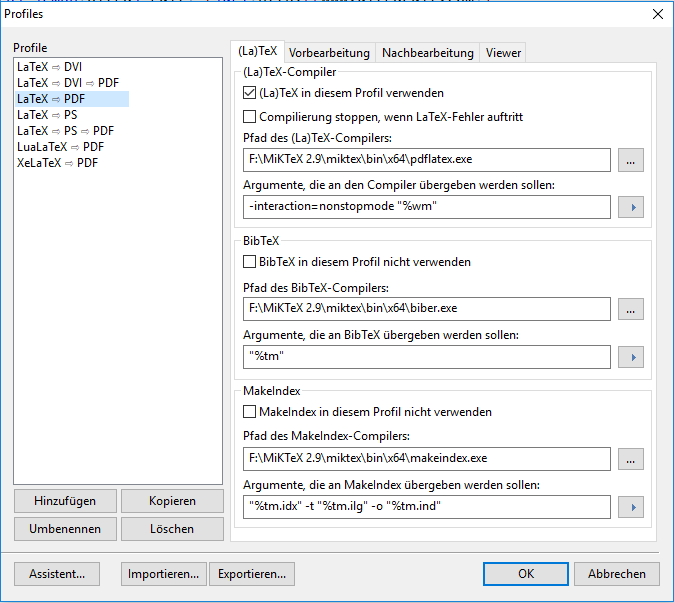
\includegraphics[width=\linewidth]{TeXnicCenterEinstellungen.PNG}
    \caption{Einstellungen für pdflatex, biber und makeindex}
		\end{subfigure}\hfill
    \begin{subfigure}[t]{0.45\textwidth}
        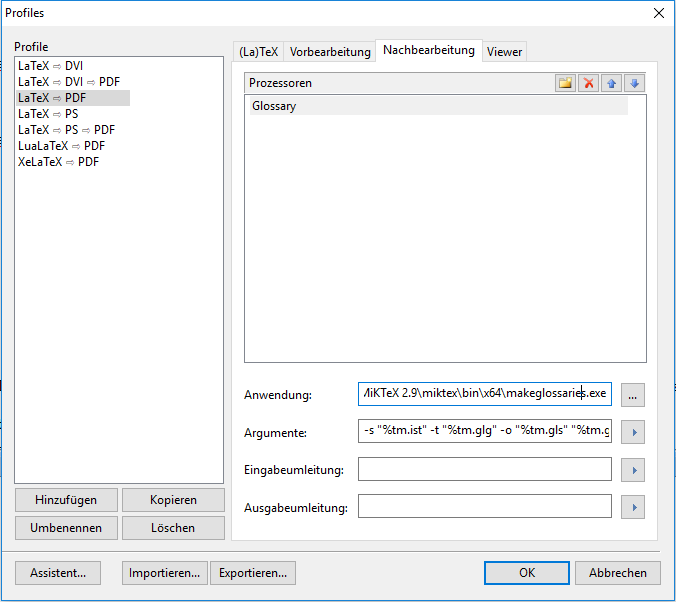
\includegraphics[width=\linewidth]{TeXnicCenterEinstellungenGlossar.PNG}
    \caption{Einstellungen für makeglossaries}
		\end{subfigure}
		\caption{Einstellungen für TeXnicCenter}
    \label{fig:Settings}
\end{figure}

\subsubsection{Mac~OS}

Unter Mac~OS wird die aktuelle Vorlage mangels verfügbarer Geräte nicht getestet. Der folgende Text bezieht sich auf die alte Vorlage und ist möglicherweise nicht mehr korrekt.

Bewährte und weit verbreitete Frontends für den Mac sind \emph{MacTeX}%
\footnote{\url{http://www.tug.org/mactex} -- enthält eine komplette und fertig
konfigurierte \latex\-Installation für Mac~OS\index[allgemein]{Mac~OS} (ca.\ 1.15 GB download).}
und \emph{TeXShop},%
\footnote{\url{http://www.uoregon.edu/~koch/texshop/}}
das üblicherweise zusammen mit der TeX-Distribution \emph{TeX Live} verwendet wird. 
Weit verbreitet ist auch der \emph{TeXworks} Editor, der ebenfalls im MacTeX Package enthalten ist und auch MiKTeX unter Windows beigefügt ist.

Weitere aktuelle Informationen zu der Arbeit mit \latex\ unter Mac~OS finden sich auf den Informationsseiten zu \latex\ der Technischen Universität Graz.\footnote{\url{http://latex.tugraz.at/programme/mac_os_x}}

\subsubsection{Linux}

Auch unter \gls{Linux}\index[allgemein]{Linux}  ist \emph{TeX Live} (\so) eine häufig verwendete TeX-Distri\-bution. 
Als Frontend sind beispielsweise
\emph{Texmaker}\footnote{\url{http://www.xm1math.net/texmaker}}(empfohlen) \emph{Lyx}\footnote{\url{http://www.lyx.org}},
\emph{Kile}\footnote{\url{http://kile.sourceforge.net}} und
verbreitet.
In manchen gängigen Linux-Versionen ist bereits eine komplette \latex-Distribution enthalten, sodass im besten Fall überhaupt keine zusätzliche Installation notwendig ist.  


Eine interessante Alternative ist die Verwendung von
\emph{Eclipse}\footnote{\url{http://www.eclipse.org}} als plattformunabhängiges Frontend 
(mit dem \emph{TeXlipse}\footnote{\url{http://texlipse.sourceforge.net}}
Plugin).


Zum Nachinstallieren zusätzlicher \latex-Pakete die nicht in der
Standardinstallation enthalten sind gibt es für Linux ebenfalls den MikTeX
Package Manager\footnote{\url{http://wiki.ubuntuusers.de/MiKTeX_Package_Manager}}. Allerdings empfiehlt es sich meist die notwendigen Pakete statt dessen über die Softwareverwaltung der Linux-Distribution zu installieren. So kann \zB\ in Ubuntu das Paket \emph{texlive-lang-german} installiert werden um die für diese Vorlage notwendige Unterstützung der deutschen Sprache nach zu installieren.


Wer es sich einfach machen will und kein Problem mit einem größeren Download bzw. größerem Speicherverbrauch auf der Festplatte hat, kann auch einfach \emph{TeX Live} mit dem Paket \emph{texlive-full} vollständig installieren.

\subsubsection{Automatische Generierung von \latex-Code}
Bei der Erstellung von komplizierterem \latex-Code kann man sich zum Glück
einiger Hilfsmittel bedienen.

\begin{itemize}
\item \emph{Online Latex Equation
Editor}\footnote{\url{http://www.codecogs.com/latex/eqneditor.php}} ist ein
einfach zu bedienender Online Editor für mathematische Formeln.
\item \emph{Online Latex Table Editor}\footnote{\url{http://www.tablesgenerator.com/latex_tables}}
\item \emph{Writer2\latex}\footnote{\url{http://www.ooowiki.de/Writer2LaTeX}}
ist ein Export-Filter für OpenOffice-Writer mit dem jede Form von Textdokumenten in
\latex-Code umgewandelt werden kann.
\item \emph{Calc2\latex}\footnote{\url{http://www.ooowiki.de/Calc2LaTeX}} ist
ein Export-Makro für OpenOffice-Calc mit dem Tabellen für das Einfügen in \latex
erzeugt werden können.
\item \emph{Dot2Tex}\footnote{\url{http://www.fauskes.net/code/dot2tex}} ist
eine Verbindung von Graphviz nach \latex. Graphen können in \latex eingebunden werden
und die Beschriftungen mit \latex geschrieben werden.
\item \emph{gnuplot}\footnote{\url{http://www.gnuplot.info}} ist ein Programm
zur Erstellen von Diagrammen. Über das \latex-Package gnuplottex kann es direkt in
den \latex-Code integriert werden.
\end{itemize}


\subsection{Literatur}
\label{sec:literatur}

Es ist müßig, ohne geeignete Literatur mit \latex zu beginnen, selbst
als fortgeschrittener Benutzer wird man immer wieder auf Hilfe angewiesen
sein. Erfreulicherweise ist sehr viel Nützliches auch online verfügbar.
Gute Startpunkte sind \zB
%
\begin{itemize}
\item \emph{\citetitle{Schmidt01}}\footcite{Schmidt01}
\item \emph{\citetitle{Oetiker01}}\footcite{Oetiker01}
\end{itemize}
%
\noindent
Als mittlerweile bereits klassisches Handbuch zu \latex ist
%
\begin{itemize}
  \item \emph{\citetitle{Kopka98}}\footcite{Kopka98}
\end{itemize}
%
zu empfehlen, zu dem es für Interessierte auch zwei vertiefende
Zusatzbände in Deutsch gibt. Zahlreiche weitere Dokumente zu
\latex und verwandten Themen finden sich \ua im Rahmen des {\em
Comprehensive TeX Archive Network} (CTAN) auf
\begin{quote}
	\url{http://www.ctan.org}%
	\footnote{\url{http://www.ctan.org/tex-archive/help/Catalogue/bytopic.html}}\newline
	\url{http://dante.ctan.org}%
	\footnote{\url{http://dante.ctan.org/tex-archive/help/Catalogue/bytopic.html}}\newline
	\url{http://www.tex.ac.uk}
\end{quote}
%
Besonders nützlich sind auch die
\emph{Comprehensive List of {\rm \latex} Symbols} \footcite{Pakin01}
und die Beschreibungen wichtiger \latex-Pakete, wie
%
\begin{quote}
	\texttt{babel} \footcite{Braams2008},\newline
  \texttt{grahics}, \texttt{graphicx} \footcite{Carlisle99},\newline
  \texttt{fancyhdr} \footcite{Oostrum97},\newline
  \texttt{caption} \footcite{Sommerfeldt07},\newline
  \texttt{subcaption} \footcite{Cochran95}.
\end{quote}


Und zu guter Letzt für die Freunde von Wikipedia gibt es noch ein \latex-Buch in der WikiBooks-Sammlung.\footnote{\url{https://en.wikibooks.org/wiki/LaTeX}}


\section{Schrift}

\subsection{Schriftarten}

\latex verwendet normalerweise die Schriften der \emph{Computer
Modern}
(CM) Serie, die so wie die \emph{TeX}-Software selbst von Donald Knuth%
\footnote{\url{http://www-cs-staff.stanford.edu/~knuth/}} entwickelt
wurden. Die drei Basis-Schrifttypen der CM-Serie in \latex sind
%
\begin{quote}
\begin{tabular}{lcl}
\textrm{Roman}      & & \verb!\textrm{Roman}!\\
\textsf{Sans Serif} & & \verb!\textsf{Sans Serif}!\\
\texttt{Typewriter} & & \verb!\texttt{Typewriter}!\\
\end{tabular}
\end{quote}
%
\noindent In den Augen vieler Benutzer ist allein die Qualität und
Zeitlosigkeit dieser Schriften ein Grund, \latex für seriöse
Zwecke zu verwenden. Ein weiterer Vorteil der \emph{TeX}-Schriften
ist, dass die unterschiedlichen Schriftfamilien und Schnitte
bezüglich der Größe sehr gut aufeinander abgestimmt sind, was %
beim Arbeiten mit verschiedenen \emph{TrueType}-Schriften (\zB\ in
\emph{Word}) durchaus zum Problem werden kann (\sa\ Kap.\
\ref{chap:Word}).

Darüber hinaus können aber in \latex auch beliebige 
\emph{PostScript}-Schrif\-ten (Type 1) verwendet werden, was allerdings in
der Praxis einiges an "`Tuning"'-Arbeit verlangt. Häufig verwendet
werden \zB\ \emph{Times} und \emph{Palatino}, derzeit ist aber ein Trend 
zurück zu den klassischen CM-Schriften zu beobachten.



\subsection{Texte hervorheben}

Texte können auf unterschiedliche Weise aus dem Fließtext hervorgehoben werden.
\begin{itemize}
%
\item Die Auszeichnung in \textit{Kursivschrift} oder "`italic"' (\verb!\textit{..}!) ist \va\ zum Hervorheben von
Betonungen und Zitaten geeignet, aber auch für
Produktbezeichnungen, Fremdwörter und Variablen im Text, \zB
%
\begin{quote}
\verb!\textit{Variable}! $\rightarrow$ \textit{Variable}
\end{quote}
%
\item {\sl Slanted} %
(\verb!\textsl{..}!) bedeutet eine geneigte Schrift und
unterscheidet sich damit deutlich von \textit{Italic}. Wird
beispielsweise verwendet für die laufenden Kopfzeilen,
Produktbezeichnungen und Markennamen -- zum Vergleich:
%
\begin{quote}
\verb!\textrm{Daimler-Chrysler}! $\rightarrow$ \textrm{Daimler-Chrysler} \newline%
\verb!\textsl{Daimler-Chrysler}! $\rightarrow$ \textsl{Daimler-Chrysler} \newline%
\verb!\textit{Daimler-Chrysler}! $\rightarrow$ \textit{Daimler-Chrysler}
\end{quote}
%
\item \textbf{Boldface} (\verb!\textbf{..}!) wird \ia\ verwendet für 
\textbf{Überschriften}, Bezeichnungen von \textbf{Abbildungen} und 
\textbf{Tabellen}, im Fließtext aber selten:
%
\begin{quote}
\verb!\textbf{Überschriften}! $\rightarrow$ \textbf{Überschriften}
\end{quote}
%
\item \emph{Emphasize} (\verb!\emph!) %
ist normalerweise gleichbedeutend mit \verb!\textit!, wobei
\verb!\emph{..}! allerdings auch bei geschachtelten
Hervorhebungen und im Bereich anderer Schriftschnitte das
"`Richtige"' tut: 
%
\begin{quote}
\setlength{\tabcolsep}{0pt}%
\begin{tabular}{lcl}
\verb!\textrm{Du \emph{auch} hier?}! & $\;\rightarrow\;$ &
    \textrm{Du \emph{auch} hier?}
\\
\verb!\textit{Du \emph{auch} hier?}! & $\;\rightarrow\;$ &
    \textit{Du \emph{auch} hier?} 
\\
\verb!\textsl{Du \emph{auch} hier?}! & $\;\rightarrow\;$ & 
    \textsl{Du \emph{auch} hier?}
\\
\verb!\textbf{Du \emph{auch} hier?}! & $\;\rightarrow\;$ & 
    \textbf{Du \emph{auch} hier?}
\\
\verb!\texttt{Du \emph{auch} hier?}! & $\;\rightarrow\;$ & 
    \texttt{Du \emph{auch} hier?}
\end{tabular}
\end{quote}
%
\item \underline{Unterstreichungen} sind ein Relikt aus der 
Schreibmaschinenära und im modernen Schriftsatz
eigentlich \underline{überflüssig}. Sie sollten daher nur in
Ausnahmefällen verwendet werden, \zB
%
\begin{quote}
\verb!\underline{überflüssig}!%
\footnote{Unterstrichene Texte werden zudem nicht automatisch abgeteilt.}
\end{quote}
%
\end{itemize}



\section{Textstruktur}

\subsection{Absatztrennung}

Absätze werden in {\latex}-Quelltext ausschließlich durch das
Einfügen einer oder mehrerer \textbf{Leerzeilen} voneinander
getrennt, es sind also \emph{keinerlei sonstige Steueranweisungen}
notwendig!
%
\begin{center}
\setlength{\fboxrule}{0.2mm}
\setlength{\fboxsep}{2mm}
\fbox{%
\begin{minipage}{0.9\textwidth}
Besonders die Verwendung von \texttt{\textbackslash\textbackslash} und 
 \texttt{\textbackslash{newline}}
Anweisungen zur Absatztrennung ist ein häufig zu beobachtender \textbf{Fehler}. 
Vor normalen Absätzen auch \emph{nichts} verloren hat die
Anweisung \texttt{\textbackslash{paragraph}\{\}}
-- sie ist in \latex\ (im Unterschied zu HTML)
eine Markierung für Überschriften mit Titel (\su)!
\end{minipage}}
\end{center}

Üblicherweise wird durch {\latex} zwischen aufeinander folgenden Ab\-sätzen
\emph{kein} zusätzlicher vertikaler Abstand eingefügt. \footnote{Das ist die
Standardeinstellung in {\latex} und natürlich abhängig von der verwendeten Dokumentenklasse, Style
etc.} 
Allerdings wird die
\emph{erste} Zeile jedes Absatzes (mit Ausnahme des ersten Absatzes
eines Abschnitts) eingerückt, um so die Absatzgrenzen deutlich zu
machen. Dieses Schema hat sich nicht nur im traditionellen
Buchsatz bewährt%
\footnote{Wer es nicht glaubt, sollte sein Bücherregal (oder notfalls das seiner Eltern) nach Gegenbeispielen durchsuchen.}
und sollte auch beibehalten werden, es sei denn
man hat wirklich \emph{sehr} gute Gründe dagegen.
Für alle übrigen Gliederungen im vertikalen Textfluss sind Überschriften (s.\ unten) vorgesehen.

\SuperPar 
Manchmal besteht allerdings der Wunsch, etwa zur Verdeutlichung eines inhaltlichen Sprungs \emph{zwischen} zwei Absätzen einen zusätzlichen Abstand einzufügen, ohne dabei eine neue Überschrift zu setzen. Das kann man gegebenenfalls (wie vor dem aktuellen Absatz passiert) durch 
%
\begin{quote}
\texttt{{\bs}SuperPar} \emph{Manchmal besteht allerdings der Wunsch, \ldots}
\end{quote}
%
erreichen, sollte jedoch sehr sparsam und wirklich \textbf{nur in begründbaren Einzelfällen} verwendet werden.%
\footnote{Das Makro \texttt{{\bs}SuperPar} ist in \texttt{htl.sty} definiert.}




\subsection{Überschriften}
\label{sec:ueberschriften}

\latex\ bietet -- abhängig von der verwendeten Dokumentenklasse --
einen Satz vordefinierter Überschriftformate in folgender Ordnung:
%
\begin{quote}
\verb!\part{!\texttt{\em Titel}\verb!}!%
\footnote{\texttt{part} ist für die Gliederung eines
größeren Werks in mehrere Teile vorgesehen und wird üblicherweise
bei einer Diplomarbeit (und auch in diesem Dokument) nicht
verwendet.}
\newline%
\verb!\chapter{!\texttt{\em Titel}\verb!}! \newline%
\verb!\section{!\texttt{\em Titel}\verb!}! \newline%
\verb!\subsection{!\texttt{\em Titel}\verb!}! \newline%
\verb!\subsubsection{!\texttt{\em Titel}\verb!}! \newline%
\verb!\paragraph{!\texttt{\em Titel}\verb!}! \newline%
\verb!\subparagraph{!\texttt{\em Titel}\verb!}!
\end{quote}
%

\paragraph{Häufiger Fehler:} Bei \verb!\paragraph{}! und
\verb!\subparagraph{}! läuft -- wie in diesem Absatz zu sehen --
der dem Titel folgende Text ohne Umbruch in der selben Zeile
weiter, weshalb man im Titel auf eine passende Punktuation (hier
\zB\ \underline{\texttt{:}}) achten sollte. Der horizontale Abstand
nach dem Titel allein würde diesen als Überschrift nicht erkennbar
machen.


\subsection{Listen}

Listen sind ein beliebtes Mittel zur Textstrukturierung. In
\latex\ sind -- ähnlich wie in HTML -- drei Arten von formatierten
Listen verfügbar: ungeordnete Auflistung ("`Knödelliste"'),
geordnete Auflistung (Aufzählung) und Beschreibungsliste
(Description):
%
\begin{verbatim}
    \begin{itemize}     ... \end{itemize}
    \begin{enumerate}   ... \end{enumerate}
    \begin{description} ... \end{description}
\end{verbatim}
%
Listeneinträge werden jeweils mit \verb!\item! markiert, bei {\tt
description}-Listen mit \verb!\item[!\texttt{\em titel}\verb!]!. Listen
können ineinander verschachtelt werden, wobei sich bei {\tt
itemize}- und \texttt{enumerate}-Listen die Aufzählungszeichen mit
der Schachtelungstiefe ändern (Details dazu in der
\latex-Dokumentation).


\subsection{Absatzformatierung und Zeilenabstand}

Diplomarbeiten werden -- wie Bücher -- in der Regel einspaltig und
im Blocksatz formatiert, was für den Fließtext wegen der großen
Zeilenlänge vorteilhaft ist. Innerhalb von Tabellen kommt es
wegen der geringen Spaltenbreite jedoch häufig zu Problemen mit
Abteilungen und Blocksatz, weshalb man dort ohne schlechtes
Gewissen zum Flattersatz ("`ragged right"') greifen sollte (wie
\zB\ in Tab.~\ref{tab:synthesis-techniques} auf Seite
\pageref{tab:synthesis-techniques}).

\subsection{Fußnoten}
Fußnoten können in \latex\ an beinahe jeder beliebigen Stelle,
jedenfalls aber in normalen Absätzen, durch die Anweisung
%
\begin{quote}
\verb!\footnote{!\texttt{\em Fußnotentext}\verb!}!
\end{quote}
%
gesetzt werden. Zwischen der \verb!\footnote!-Marke und dem davor
liegenden Text sollte grundsätzlich \emph{kein Leerzeichen} entstehen (eventuelle
Zeilen\-um\-brüche mit \verb!%! auskommentieren).
Die Nummerierung und Platzierung der Fußnoten
erfolgt automatisch, sehr große Fußnoten werden notfalls sogar auf
zwei aufeinander folgende Seiten umgebrochen.


\subsubsection{Fußnoten in Überschriften}

Auch das braucht man ab und zu, ist aber \va\ deshalb kein so
einfacher Fall, weil die Fußnote in einer Überschrift nur an Ort
und Stelle auf scheinen darf, nicht aber im \emph{Inhaltsverzeichnis}! Ein
konkretes Beispiel dafür ist die Überschrift zu
Kapitel~\ref{chap:Word}, die etwa folgendermaßen definiert ist:
%
\begin{quote}
\begin{verbatim}
\chapter[Hinweise für Word-Benutzer]%
        {Hinweise für Word-Benutzer%
        \protect\footnote{Dieser Abschnitt ....}}%
\end{verbatim}
\end{quote}
%
Dabei ist der erste (optionale) Titel \verb![Hinweise für ...]!
der Eintrag im Inhaltsverzeichnis und im Seitenkopf. 
Der zweite (identische) Titel
\texttt{\{Hinweise für ...\}} erscheint auf der aktuellen Seite und
enthält auch den \verb!\footnote{}! Eintrag, der allerdings an
dieser Stelle durch die Direktive \verb!\protect! "`geschützt"'
werden muss. Die \verb!%!-Zeichen sind übrigens notwendig,
um eventuelle Leerzeichen, die durch Zeilenumbrüche im Quelltext
entstehen, zu eliminieren (diesen Trick braucht man %
in \latex\ häufig, s.\ Abschn.~\ref{sec:kommentare}). 
Ziemlich kompliziert also, und damit 
ein weiterer Grund, Fußnoten an solchen Stellen überhaupt zu vermeiden.

Generell sollte man mit Fußnoten sparsam umgehen, da sie den
Textfluss unterbrechen und den Leser ablenken. Insbesondere
sollten Fußnoten nicht (wie \va\ in manchen
sozialwissenschaftlichen Werken gepflegt) derart lang werden, dass
sie einen Großteil der Seite einnehmen und damit praktisch ein
zweites Dokument bilden.%
\footnote{Das führt bei Dokumenten mit vielen Fußnoten bei manchen Lesern angeblich so weit, dass sie aus Neugier (oder Versehen) regelmäßig bei den Fußnoten zu lesen beginnen und dann mühevoll die zugehörigen, kleingedruckten Verweise im Fließtext suchen.}


\subsection{Querverweise}
\label{sec:querverweise}

Zur Verwaltung von Querverweisen innerhalb eines Dokuments stellt
\latex\ einen sehr einfachen Mechanismus zur Verfügung. Zunächst
muss jede Stelle (Kapitel, Abschnitt, Abbildung, Tabelle etc.)
durch
%
\begin{quote}
\verb!\label{!\texttt{\em key}\verb!}!
\end{quote}
%
markiert werden, wobei \texttt{\em key} ein gültiges \latex-Symbol sein
muss. Damit Labels (die nur Zahlen sind) nicht verwechselt werden,
ist es üblich, sie je nach Bedeutung mit einer unterschiedlichen
Prefix zu versehen, \zB\
%
\begin{quote}
\tabcolsep0pt
\begin{tabular}{ll}
\verb!cha:!\texttt{\em kapitel}   & \ \ldots\ für Kapitel  \\
\verb!sec:!\texttt{\em abschnitt} & \ \ldots\ für Abschnitte (Sections) und Unterabschnitte \\
\verb!fig:!\texttt{\em abbildung} & \ \ldots\ für Abbildungen \\
\verb!tab:!\texttt{\em tabelle}   & \ \ldots\ für Tabellen \\
\verb!equ:!\texttt{\em gleichung} & \ \ldots\ für Formeln und Gleichungen\\
\end{tabular}
\end{quote}
%
\noindent Beispiele:\ \verb!\label{cha:Einleitung}! oder
\verb!\label{fig:Screen-1}!. Mit den Anweisungen
%
\begin{quote}
\verb!\ref{!\texttt{\em key}\verb!}! 
\hspace{1em} oder \hspace{1em} 
\verb!\pageref{!\texttt{\em key}\verb!}!
\end{quote}
%
kann an beliebiger Stelle im Dokument die zu \texttt{\em key} gehörige
Nummer bzw.\ Seitennummer eingesetzt werden, \zB\
%
\begin{quote}
\verb!.. wie in Kap.~\ref{cha:Einleitung} erwähnt ..!\\
\verb!.. der Screenshot auf Seite \pageref{fig:Screen-1} ..!
\end{quote}
%
Übrigens werden die Bezeichnungen \emph{Kapitel} und {\em
Abschnitt} auffallend oft falsch verwendet -- Kapitel haben
ausschließlich "`ungebrochene"' Nummern:
%
\begin{quote}
\begin{tabular}{ll}
   \textrm{Richtig:\ } & Kapitel 7 oder Abschnitt 2.3.4\\
   \textbf{Falsch:\ }  & Kapitel 7.2 oder Abschnitt 5
\end{tabular}
\end{quote}


\section{Wortabstand und Punktuation}

\subsection{\emph{French Spacing}}
Im englischsprachigen Schriftsatz ist es üblich, nach jedem
Satzende einen gegenüber dem normalen Wortzwischenraum
vergrößerten Abstand einzusetzen. Obwohl dies im Deutschen und
Französischen traditionell nicht so ist, wird es wegen der
verbesserten Lesbarkeit auch hier manchmal verwendet (nicht in diesem
Dokument). Falls man die englische ("`nicht-französische"') Satztrennung mit
zusätzlichem Abstand bevorzugt, ist lediglich die Zeile
%
\begin{quote}
\verb!\nonfrenchspacing!
\end{quote}
%
am Beginn des Dokuments einzusetzen. 
In diesem Fall sollte man 
aber die Interpunktion innerhalb von
Sätzen (nach .\ und :) sorgfältig beachten. Beispielsweise
schreibt man "`Dr.\ Mabuse"' in der Form
%
\begin{quote}
\verb!Dr.\ Mabuse! oder \verb!Dr.~Mabuse!
\end{quote}
%
Im zweiten Beispiel wird mit \verb!~! zudem ein Zeilenumbruch am Leerzeichen verhindert.


\subsection{Gedanken- und Bindestriche}
\label{sec:gedankenstrich}

Die Verwendung der falschen Strichlängen (mit und ohne
Zwischenraum) ist ganz allgemein eine häufige Fehlerquelle.
Bewusst unterscheiden sollte man zwischen
%
\begin{itemize}
\item kurzen Bindestrichen (wie in "`Wagner-Jauregg"'), %
\item Minus-Zeichen, \zB\ $-7$ (erzeugt mit \verb!$-7$!), und %
\item echten Gedankenstrichen -- wie hier (erzeugt mit \verb!--!).
\end{itemize}
%
\noindent Für das Setzen von Gedankenstrichen\footnote{Für alle
drei gibt es übrigens auch in \emph{Word} entsprechende
Sonderzeichen.} gibt es eindeutige Konventionen:
%
\begin{enumerate}
\item Im \emph{Deutschen} setzt man üblicherweise einen von zwei
Leerzeichen umgebenen Gedankenstrich%
\footnote{Halbgeviertstrich (\emph{En Dash}).} -- wie hier (in
\latex\ mit {\verb*! -- !}). Dieser wird auch für die Angabe von
Zahlenintervallen (Seiten 12--19) benutzt. 
%
\item In \emph{englischen} Texten verwendet man einen noch längeren
Gedankenstrich\footnote{Geviertstrich (\emph{Em Dash}).} \emph{ohne}
zusätzliche Leerzeichen---\emph{as we should be knowing by now}
(in \latex\ mit {\verb*!---!}).
%
\end{enumerate}




\subsection{Kommentare}
\label{sec:kommentare}


Textteile können in \latex\ zeilenweise mit \verb!%! auskommentiert werden. Der einem 
\verb!%!-Zeichen nachfolgenden Text wird bis zum nächsten Zeilenende überlesen:
%
\begin{quote}
\verb!Das wird gedruckt. %Dieser Text wird ignoriert.!
\end{quote}
%
Häufig verwendet werden Kommentarzeichen aber auch zum Ausblenden von 
\emph{white space}, also Leerzeichen und Zeilenumbrüchen.
Folgendes Beispiel zeigt etwa, wie man mit \verb!%! am Zeilendende das Entstehen
eines Leerzeichens vor einer nachfolgenden Fußnotenmarke vermeiden kann:
%
\begin{quote}
\begin{verbatim}
In Österreich isst man sonntags Schnitzel.%
\footnote{Was die allgemein gute Kondition erklärt.}
\end{verbatim}
\end{quote}
%

\begin{sloppypar}
\noindent
Auf ähnliche Weise kann man das Entstehen von ungewolltem Absatz\-zwischenraum durch 
gezielten Einsatz von Kommentarzeilen vermeiden, \zB\ vor und nach einem zentrierten
Textabschnitt:
\end{sloppypar}
%
\begin{quote}
\begin{verbatim}
... normaler Text.
%
\begin{center}
   Dieser Test ist zentriert.
\end{center}
%
Und jetzt geht es normal weiter ...
\end{verbatim}
\end{quote}
%
Darüber hinaus bietet die \verb!comment!-Umgebung die Möglichkeit, größere Text\-blöcke
in einem Stück auszublenden:
%
\begin{quote}
\begin{verbatim}
\begin{comment}
Dieser Text ...
   ... wird ignoriert.
\end{comment}
\end{verbatim}
\end{quote}




\subsection{Anführungszeichen}
\label{sec:anfuehrungszeichen}

Mit Anführungszeichen geht man aus Gewohnheit meist etwas
nachlässig um; auch dabei sind aber die Unterschiede zwischen Deutsch
und Englisch zu beachten. Hier die richtige \latex-Notation für
beide Sprachen:
%
\begin{quote}
\verb!``English''! $\rightarrow$ ``English'' \\
\verb!"`Deutsch"'! $\rightarrow$ "`Deutsch"' 
\end{quote}
%
Bei richtiger Einstellung werden beispielsweise im TeXnicCenter-Editor und im
Eclipse-Plugin Texlipse die entsprechenden Zeichenfolgen automatisch
eingesetzt. \emph{Einfache} Anführungszeichen erzeugt man im Englischen analog, im Deutschen benötigt man dafür die Makros \verb!\glq! \bzw\ \verb!\grq! (German left/right quote):
\begin{quote}
\verb!`English'! $\rightarrow$ `English' \\
\verb!{\glq}Deutsch{\grq}! $\rightarrow$ {\glq}Deutsch{\grq} 
\end{quote}





\section{Abteilen}
\label{subsec:layout-abteilen}

Um ein sauberes Schriftbild zu erreichen sind -- speziell im
Deutschen wegen der großen Wortlängen -- Abteilungen
(Silbentrennung, Hyphenation) unerlässlich, entweder manuell durch
Einfügen von optionalen Trennzeichen oder automatisch. In \latex
wird grundsätzlich automatisch abgeteilt, wobei die Sprache am
Beginn des Dokuments festgelegt und entsprechende Abteilungsregeln
für den gesamten Text verwendet werden.

Besonders bei schmalen Textspalten kann es vorkommen, dass \latex
keine geeignete Stelle für den Zeilenumbruch findet und den Text
über den rechten Rand hinaus laufen lässt. Das ist durchaus
beabsichtigt und soll anzeigen, dass an dieser Stelle ein Problem
besteht, das man durch manuelles Eingreifen reparieren muss.

Generell sollte man gegenüber der automatischen Abteilung
misstrauisch sein und das Endergebnis stets sorgfältig überprüfen.
Vor allem Wörter mit Umlauten oder Bindestrichen werden in \latex\ 
oft unrichtig abgeteilt.
Bei Bedarf kann man mit \verb!\-! gezielt zulässige Abteilungspunkte 
definieren, wie \zB\ in
%
\begin{quote}
\verb!Fach\-hoch\-schul\-kon\-fe\-renz!.
\end{quote}
%
In echten Problemfällen -- etwa bei Schwierigkeiten mit Textelementen, die nicht umgebrochen 
werden dürfen oder können -- kann man \latex\ dazu veranlassen, in einzelnen Absätzen
etwas weniger pingelig zu formatieren. Das erreicht man durch
%
\begin{quote}
\begin{verbatim}
\begin{sloppypar}
    Dieser Absatz wird ``schlampig'' (sloppy) gesetzt ...
\end{sloppypar}
\end{verbatim}
\end{quote}
%
Der letzte Rettungsanker ist, den betreffenden Absatz so umzuschreiben, dass sich ein passabler Zeilenumbruch ergibt (schließlich ist man ja selbst der Autor und niemandem eine
Rechtfertigung schuldig).%
\footnote{Angeblich waren eigenständige Textänderungen in solchen Fällen auch beim früheren Bleisatz durchaus üblich.}



\section{Das {\tt htl}-Paket}

Diesem Dokument angeschlossen sind zwei Dateien, die beide zum Erstellen dieses Dokuments erforderlich sind:
%
\begin{description}
\item[\url{htldipl.cls} (class file):] definiert die 
		Dokumentenstruktur, Layout und den gesamten Vorspann des Dokuments (Titelseite etc.).
\item[\url{htl.sty} (style file):] enthält nützliche 
		Definitionen. Diese Datei wird von \url{htldipl.cls} automatisch geladen, kann 
		aber grundsätzlich auch für andere Dokumente verwendet werden.
\end{description}


\subsection{Einstellungen}


Alle (\verb!.tex!) Dokumente dieser Klasse beginnen mit der Anweisung
%
\begin{itemize}
\item[] \verb!\documentclass[!\texttt{\emph{language,printsetting,colormode}}\verb!]{htldipl}! 
\end{itemize}
%
Mit der Option \texttt{\emph{language}} kann die Hauptsprache des Dokuments spezifiziert werden, 
die möglichen Werte dafür sind
%
\begin{itemize}
\item[] \verb!german! (\emph{default})
\item[] \verb!english!
\end{itemize}

Mit der Option \texttt{\emph{printsetting}} kann spezifiziert werden, ob das Dokument im Druck einseitig oder beidseitig gedruckt werden soll. Diese Option steuert natürlich nicht direkt den Drucker, sondern passt die Formatierung des Dokuments für den späteren Druck an. \ZB\ werden bei bedarf Leerseiten hinzugefügt, damit bei beidseitigem Druck die Kapitel immer auf der Vorderseite beginnen.
Die möglichen Werte dafür sind
%
\begin{itemize}
\item[] \verb!oneside! (\emph{default})
\item[] \verb!twoside!
\end{itemize}
%
Mit der Option \texttt{\emph{colormode}} kann spezifiziert werden, ob der im Dokument enthaltene Source-Code mit farblichem Syntax-Highlighting dargestellt werden soll oder in Grau/Schwarz. Wird das ganze Dokument auf einem Farbdrucker gedruckt empfiehlt sich die farbliche Darstellung. Werden nur die Seiten mit Farbbildern auf einem Farbdrucker gedruckt sollte für die bessere Lesbarkeit des Codes die andere Darstellung gewählt werden.
Die möglichen Werte dafür sind
%
\begin{itemize}
\item[] \verb!color! (\emph{default})
\item[] \verb!black!
\end{itemize}
%
Der vollständige Quelltext für eine entsprechende \verb!.tex! Hauptdatei ist in Anhang \ref{app:latex} 
gelistet.


\subsubsection{Angaben zur Arbeit}

Zum erstellen der Titelseite sind einige Angaben notwendig \zB\:
%
\begin{itemize}
\item[] %
\verb!\title{!\texttt{\em Titel der Arbeit}\verb!}! \newline%
\verb!\abteilung{!\texttt{\em Abteilung}\verb!}! \newline%
\verb!\studienort{!\texttt{\em Studienort}\verb!}! \newline%
\verb!\abgabejahr{!\texttt{\em Jahr der Abgabe}\verb!}!
\end{itemize}
%

Da die Diplomarbeit von einer unterschiedliche Anzahl von Autoren geschrieben werden kann, können bei den Angaben zu den Autoren die nicht benötigten Einträge einfach frei gelassen werden.


\subsubsection{Titelseiten}

Die ersten Seiten der Arbeit, einschließlich der Titelseite,
werden durch die Anweisung
\begin{itemize}
\item[] %
\verb!\maketitle!  
\end{itemize}
automatisch generiert, abhängig von den obigen
Einstellungen:
%
\begin{center}
\begin{tabular}{cll}
\emph{Seite} & \emph{Diplomarbeit} \\
  \hline
  {\rm i} & Titelseite \\
  {\rm ii} & Eidesstattliche Erklärung \\
  \hline
\end{tabular}
\end{center}






\subsection{Definierte Abkürzungen}

Es wird im \texttt{htl}-Paket weiters eine Reihe von Abkürzungsmakros%
\footnote{In Anlehnung an den \texttt{jkthesis}-Style von Jochen
Küpper (\url{http://www.jochen-kuepper.de}).} definiert, die das
Schreiben vereinfachen und für konsistente
Zwisch\-en\-ab\-stän\-de sorgen (Tab.~\ref{tab:abkuerzungen}).
Bei der Verwendung von Makros ist allgemein zu beachten, dass sie nachfolgende Leerzeichen bisweilen "`auffressen"', sodass vor dem nachfolgenden Text kein Abstand erzeugt wird.%
\footnote{Bei den meisten der in \texttt{htl.sty} definierten Makros wird dies
allerdings durch den Einsatz von \texttt{\textbackslash xspace} verhindert.} Dagegen kann man sich mit \verb!\!-Zeichen oder \verb!{}! behelfen, wie in folgendem 
(nicht sehr schönen) Beispiel:
%
\begin{itemize}
\item[] \verb!Mopeds und Autos haben \ia\ zwei {\bzw} vier Räder.!\\
      Mopeds und Autos haben \ia\ zwei {\bzw} vier Räder.
\end{itemize}


\begin{table}
\caption{In \texttt{htl.sty} definierte Abkürzungsmakros.}
\label{tab:abkuerzungen}
\centering
\begin{tabular}{llp{2cm}ll}
\hline
    \verb+\bzw+        & \bzw   & &  \verb+\ua+         & \ua \\
    \verb+\bzgl+       & \bzgl  & &  \verb+\Ua+         & \Ua \\
    \verb+\ca+         & \ca    & &  \verb+\uae+        & \uae \\
    \verb+\dah+        & \dah   & &  \verb+\usw+        & \usw \\
    \verb+\Dah+        & \Dah   & &  \verb+\uva+        & \uva \\
    \verb+\ds+         & \ds    & &  \verb+\uvm+        & \uvm \\
    \verb+\evtl+       & \evtl  & &  \verb+\va+         & \va \\
    \verb+\ia+         & \ia    & &  \verb+\vgl+        & \vgl \\
    \verb+\sa+         & \sa    & &  \verb+\zB+         & \zB \\
    \verb+\so+         & \so    & &  \verb+\ZB+         & \ZB \\
    \verb+\su+         & \su    & &                     &     \\
\hline
\end{tabular}
\end{table}




\subsection{Sprachumschaltung}
\label{sec:sprachumschaltung}

Für englischsprachige Abschnitte (\zB\ das Abstract oder englische
Zitate) sollte die \emph{Sprache} von Deutsch auf Englisch
umgeschaltet werden, um die richtige Form der Silbentrennung zu
erhalten. Damit man nicht versehentlich auf das Rückstellen der
Sprache vergisst, sind dafür im \texttt{htl}-Paket zwei
spezielle \emph{Environments} vorgesehen:
%
\begin{itemize}
\item[] 
\verb!\begin{english}!\\
\verb!    This is a 1-page (maximum) summary!\\
\verb!    of your work in English.!\\
\verb!\end{english}!
\end{itemize}

\begin{itemize}
\item[] 
\verb!\begin{german}!\\
\verb!    Text in Deutsch (wenn die Hauptsprache!\\
\verb!    auf Englisch gesetzt ist).!\\
\verb!\end{german}!
\end{itemize}
%
Zur Kontrolle lässt sich aktuelle Spracheinstellung übrigens mit dem Makro \verb!\languagename!
anzeigen. An dieser Stelle ergibt das beispielsweise "`\texttt{\languagename}"' (\emph{new german}, \dah\ neue deutsche Rechtschreibung).


\subsection{Zusätzliche {\latex}-Pakete}

Für die Verwendung dieses Dokuments ist eine Reihe von
zusätzlichen \latex-Paketen erforderlich
(Tab.~\ref{tab:packages}). Diese Pakete werden am Anfang
durch das \texttt{htl}-Paket automatisch geladen. 
Alle verwendeten Pakete sind
Teil der \latex\ Standard-Installation, wie \zB in MikTeX, wo
man auch entsprechende Dokumentation findet (meist als DVI-Dateien).
Die aktuellen Versionen der Pakete sind online verfügbar, \ua\ auf den
in Abschn.~\ref{sec:literatur} angegebenen CTAN-Sites.

\begin{table}
\caption{Im \texttt{htl}-Paket verwendeten \latex-Ergänzungen. Alle sind in
gängigen \latex\ Standardinstallationen (\zB MikTeX) bereits enthalten.}
\label{tab:packages}
\centering\small
\tabcolsep2pt
\begin{tabular}{ll}
%\hline
\emph{Paket} &  \emph{Funktion} \\
\hline
\texttt{algorithmicx} & Beschreibung von Algorithmen \\ 
\texttt{amsfonts}, \texttt{amsbsy}   &  Mathematische Symbole \\ 
\texttt{amsmath}  &  Mathematischer Schriftsatz \\ 
\texttt{babel}  	&  Sprachumschaltung \\ 
\texttt{babelbib} &  Mehrsprachige Literaturverwaltung \\ 
\texttt{caption}  &  Flexiblere Captions \\ 
\texttt{cite}     &  Sortierte Literaturverweise \\ 
\texttt{color}    &  Farbige Textelemente und Hintergrundfarben \\ 
%\texttt{eurosym}  &  {\euro}-Symbol (\verb!\euro!)\\ 
\texttt{marvosym}  &  {\euro}-Symbol (\verb!\euro!)\\ 
\texttt{exscale}  &  Korrekte Schriftgrößen im Math-Modus \\ 
\texttt{fancyhdr} &  zur Gestaltung Kopfzeilen (header) \\ 
\texttt{float}    &  Verbessertes Float-Handling \\ 
\texttt{fontenc}  &  zur Verwendung der cm-super Type1 Postscript Schriften \\ 
\texttt{graphicx} &  Einbindung von EPS-Grafiken \\ 
\texttt{hyperref} &  erzeugt aktive Querverweise im PDF-Dokument \\ 
\texttt{ifthen}   &  für logische Entscheidungen in \latex\\
\texttt{inputenc} &  Erweiterter Eingabezeichensatz \\ 
%\texttt{latin1}   &  T1-Schriften, \ua zur besseren Silbentrennung \\ 
\texttt{listings-utf8} &  Auflistung von Programmcode \\ 
\texttt{pdfpages}  &  PDF-Seiten in das Dokument einbinden \\ 
\texttt{upquote}  &  Gerade Hochkommas in \texttt{verbatim}-Texten \\ 
\texttt{url}      &  Behandlung von URLs im Text \\ 
\texttt{verbatim} &  Verbesserte \texttt{verbatim}-Umgebung \\
\hline
\end{tabular}
\end{table}





\section{\latex-Fehlermeldungen und Warnungen}

Während des Durchlaufs gibt \latex\ Unmengen von
Meldungen aus, die einen in ihrer Fülle zunächst nicht verwirren
sollten, \zB:

\begin{scriptsize}
\begin{verbatim}
...
Overfull \hbox (14.43593pt too wide) in paragraph at lines 105--109
\OT1/cmr/m/n/10.95 F[]ur die Ein-bin-dung von Gra-phi-ken in L[]T[]X wird die V
er-wen-dung des Standard-
[10] [11]
Overfull \hbox (5.01222pt too wide) in paragraph at lines 148--154
\OT1/cmr/m/n/10.95 wen-di-gen Ras-te-rung kei-nen Sinn, auch bei 1200 dpi-Druck
ern. Spe-zi-ell \OT1/cmr/m/it/10.95 Screen-
...
\end{verbatim}
\end{scriptsize}
%
\emph{Errors} (Fehler) müssen korrigiert werden, wobei einem \latex\ diese Arbeit 
nicht leicht macht, da manchmal (\zB\ wenn eine schließende Klammer \verb!}! 
vergessen wurde) das Problem erst viel später im Text lokalisiert wird.
In solchen Fällen kann es nützlich sein, das erzeugte Ausgabedokument
zu inspizieren um festzustellen, ab welcher Stelle die Ergebnisse
aus dem Ruder laufen.  
Bei kapitalen Fehlern bleibt der \latex-Prozessor überhaupt stehen und 
erzeugt keine Ausgabe (in Verbindung mit einer meist kryptischen
Fehlermeldung) -- hier hilft meist nur eine genaue
Analyse des Quelltexts oder der gerade zuvor durchgeführten Schritte.
Ein ausführliches Fehlerprotokoll findet man jeweils in der \verb!.log!-Datei 
des Hauptdokuments.

Falls keine Fehler mehr angezeigt werden, ist zumindest die syntaktische Struktur
des Dokuments in Ordnung.
Genauer ansehen sollte man sich die Liste von Meldungen jedoch
spätestens beim Abschluss der Arbeit, um übrig gebliebene Probleme, wie
überlange Textzeilen, unaufgelöste Verweise und ähnliche zu
beseitigen.
Am Ende sollte das Ergebnis jedenfalls so ausehen:
%
\begin{quote}
\verb!LaTeX-Result: 0 Error(s), 0 Warning(s), ...!
\end{quote}